% 第5章第5节：树分解的构造（由消元次序构造、最小度与最小填充、弦图与完美消元序、团树与最大权生成树）。

\section{树分解的构造}
\label{sec:graph-tree-decomposition-construction}

上一节给出了树分解的合法性条件，但没有说明怎样得到一个分解。本节先说明，任何一个完整的消元次序都能机械地产生一个树分解，其宽度就是该次序下最大的中间作用域；再讨论没有给定次序时怎样选择次序。最后考虑一类不需要补边的图，即弦图，在其上可以直接用极大团作袋，并用第~\ref{sec:graph-minimum-spanning-tree}节的最大权生成树把它们连成团树。与第~\ref{sec:graph-variable-elimination}节不同，本节只做结构上的操作：输出袋和袋之间的连接，不计算任何成本表。

\subsection{基于消元次序的构造}

\paragraph{逐轮记录袋}
输入非空有限无向图$\mathcal G=(V,E)$和一个包含每个顶点恰好一次的消元次序$\pi$。按$\pi$逐个处理顶点：处理$v$时，读出$v$在当前图中的邻居集合，记为$N^+_\pi(v)$（上标$+$表示这些邻居都在次序中排在$v$之后）；记录袋$B_v=\{v\}\cup N^+_\pi(v)$；把$N^+_\pi(v)$中的顶点两两连边，然后删去$v$及其关联边。这正是第~\ref{sec:graph-variable-elimination}节中消元在原始图上的结构操作，袋$B_v$就是消去$x_v$时同时处理的变量组。

关键在于每一轮都要从更新后的图读取邻居。图~\ref{fig:graph-dp-elimination-to-decomposition}的例子有边$\{1,2\},\allowbreak\{1,4\},\allowbreak\{2,3\},\allowbreak\{3,4\},\allowbreak\{3,5\},\allowbreak\{4,5\}$，次序为$(1,2,5,3,4)$。处理$1$时，邻居$2,4$不相邻，补入填充边$\{2,4\}$，记袋$\{1,2,4\}$。处理$2$时，当前邻居是$\{3,4\}$，其中$4$是刚补入的邻居，记袋$\{2,3,4\}$。若误从原图读取，$2$的剩余邻居只有$3$，袋$\{2,3\}$就漏掉了消去$x_1$后新函数同时读取的$x_2,x_4$。随后依次记袋$\{3,4,5\}$、$\{3,4\}$、$\{4\}$，不再需要补边。

\paragraph{连接父袋}
袋记录完毕后，对每个$N^+_\pi(v)$非空的顶点$v$，令$p(v)$为$N^+_\pi(v)$中在次序里最早的顶点，把$B_v$连到$B_{p(v)}$；$N^+_\pi(v)$为空的袋没有父袋，作为根。原图不连通时会有多个根，可以再用任意边把这些根连成一棵树，这些边的接口为空。在上例中$p(1)=2$、$p(2)=3$、$p(5)=3$、$p(3)=4$，得到以$B_4=\{4\}$为根的袋树，最大袋含$3$个顶点，宽度为$2$。

\begin{figure}[!htb]
  \centering
  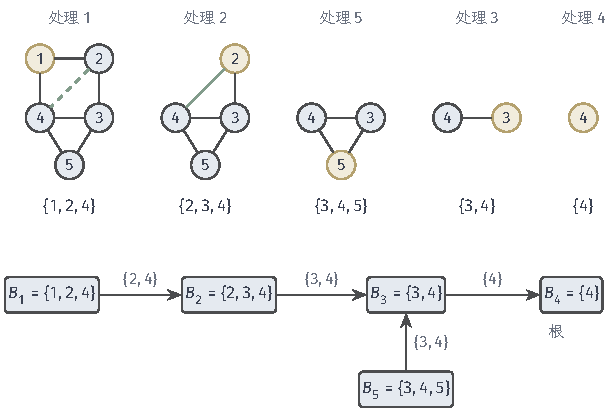
\includegraphics[width=104.369mm]{figures/01-basic-mathematics/04-graphs/tikz/c5-elimination-to-decomposition/figure.pdf}
  \caption{由消元次序$(1,2,5,3,4)$构造树分解。上行：每一轮的当前图，黄色为正在处理的顶点，绿色虚线为本轮补入的填充边，下一轮中它以绿色实线留在当前图里；图下标出记录的袋。下：按“连到最早被处理的后续邻居”连接父袋得到的袋树，箭头指向父袋，边旁标出接口。}
  \label{fig:graph-dp-elimination-to-decomposition}
\end{figure}

下面的定理说明这样得到的结构总是树分解。消元次序$\pi$下的最大后续邻居数$\max_v|N^+_\pi(v)|$称为$\pi$的\term{诱导宽度}（induced width）。

\begin{theorem}[消元次序产生树分解]
\label{thm:graph-dp-elimination-decomposition}
设$\mathcal G$是非空有限无向图，$\pi$是它的完整消元次序。按上面的方法记录袋$B_v=\{v\}\cup N^+_\pi(v)$并连接父袋（多个根之间用空接口边连接），得到的是$\mathcal G$的树分解，其宽度等于$\pi$的诱导宽度。因此$\mathcal G$的树宽不超过任何消元次序的诱导宽度。
\end{theorem}

\begin{proof}
先说明袋树是树。每个非根袋恰有一条通向父袋的边，而父点$p(v)$在次序中排在$v$之后，沿父边前进时次序位置严格增大，所以不会回到出发点，不形成环。每条父链都在有限步后到达一个根，各根之间再用树边连接，整体连通且无环。

顶点覆盖由$v\in B_v$给出。边覆盖：设$\{u,v\}\in E$且$u$先于$v$被处理。在处理$u$之前，图中只删去过已处理的顶点及其关联边，所以边$\{u,v\}$仍在，$v\in N^+_\pi(u)$，于是$B_u$同时含$u,v$。

运行交集：设$z\in B_v$且$v\neq z$，只需证明从$B_v$沿父链向上的每个袋都含$z$，直到到达$B_z$；这样含$z$的每个袋都与$B_z$由一条全部含$z$的路径相连，$T_z$连通。由于$z\in N^+_\pi(v)$，父点$p(v)$要么就是$z$，要么排在$z$之前。若$p(v)\neq z$，处理$v$时$z$与$p(v)$都是$v$的邻居，补团操作使它们相邻；在处理$p(v)$之前$z$没有被删除，这条边仍在，所以$z\in N^+_\pi(p(v))\subseteq B_{p(v)}$。对$p(v)$重复同样的论证，次序位置严格增大，最终到达$B_z$。

宽度为$\max_v|B_v|-1=\max_v|N^+_\pi(v)|$，即诱导宽度。树宽是全部树分解宽度的最小值，所以不超过它。
\end{proof}

证明中的边覆盖论证同样适用于填充边，因此所得袋树也是补边后图的树分解。构造的结构开销可以分开报告：设处理第$t$个顶点时它有$d_t$个当前邻居，补边要检查$\sum_t d_t(d_t-1)/2$对顶点，记录的袋共含$\sum_t(d_t+1)$个顶点；用支持常数时间查边和加边的邻接集合实现时，时间为$O\bigl(n+m+\sum_t d_t^2\bigr)$。这只是结构操作的开销；第~\ref{sec:graph-bag-dp}节在袋上计算成本表时，开销随袋大小指数增长，需要另算。

\subsection{消元次序的选择}

定理~\ref{thm:graph-dp-elimination-decomposition}把找好的树分解归结为找诱导宽度小的消元次序。在一般图上找最优次序是困难的，实践中常用局部规则每轮挑选一个顶点。两条常见规则是：\term{最小度启发式}（min-degree），选当前邻居最少的顶点；\term{最小填充启发式}（min-fill），选消去时需要补边最少的顶点，即当前邻域中缺少的边数最少者。

\begin{algorithm}[贪心选择消元次序]
\label{alg:graph-dp-greedy-order}
输入：非空有限无向图和一条评分规则（当前度数或当前缺边数）。输出：消元次序、各轮的袋和填充边。
\begin{enumerate}
  \item 对当前图中的每个顶点按规则计算评分，取评分最小者，评分相同时取编号最小者，记为$v$。
  \item 记录袋$\{v\}\cup N(v)$，把$N(v)$补成团，删去$v$，并把$v$追加到次序末尾。
  \item 若图非空，回到第1步，并在更新后的图上重新计算评分。
\end{enumerate}
\end{algorithm}

评分必须在每轮更新后的图上重算。若只按初始度数排一次序，或用原图的缺边数代替当前缺边数，得到的就不是这两条规则，因为补边会改变其他顶点的度数和邻域。

\paragraph{同一图上的两种评分}
图~\ref{fig:graph-dp-min-degree-min-fill}的图有六个顶点和边$\{1,3\},\allowbreak\{1,4\},\allowbreak\{1,5\},\allowbreak\{1,6\},\allowbreak\{2,3\},\allowbreak\{2,4\},\allowbreak\{2,6\},\allowbreak\{3,5\},\allowbreak\{4,5\},\allowbreak\{5,6\}$。初始度数依次为$4,3,3,3,4,3$；缺边数依次为$3,3,2,2,3,2$，例如顶点$2$的邻居$3,4,6$两两不相邻，缺$3$条边，而顶点$3$的邻居$1,2,5$中只缺$\{1,2\}$与$\{2,5\}$。最小度规则在度数为$3$的$2,3,4,6$中按编号选$2$，补入$\{3,4\},\allowbreak\{3,6\},\allowbreak\{4,6\}$；此后剩下的五个顶点度数都是$4$，选$1$时袋为$\{1,3,4,5,6\}$，宽度升到$4$。最小填充规则先选缺边最少的$3$，补入两条边，袋为$\{1,2,3,5\}$；其后依次选$4,1,2,5,6$，不再补边，最大袋含$4$个顶点，宽度为$3$。

\begin{figure}[!htb]
  \centering
  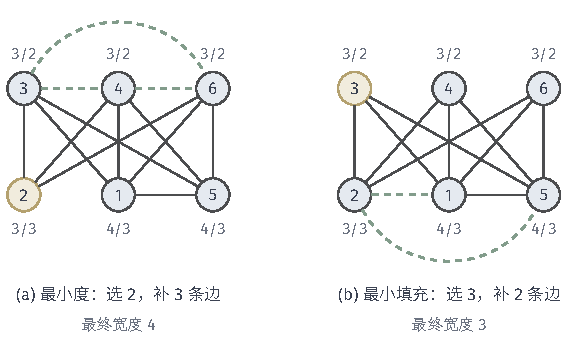
\includegraphics[width=96.778mm]{figures/01-basic-mathematics/04-graphs/tikz/c5-min-degree-min-fill/figure.pdf}
  \caption{最小度规则与最小填充规则的第一步。每个顶点旁的“$d/f$”是当前度数与当前缺边数。左：最小度规则在度数为$3$的顶点中按编号选$2$（黄色），要补三条绿色虚线，最终宽度为$4$。右：最小填充规则选缺边最少的$3$（黄色），只补两条边，最终宽度为$3$。}
  \label{fig:graph-dp-min-degree-min-fill}
\end{figure}

\paragraph{启发式只给出上界}
两种规则都只看一步：度数小不代表补边少，补边少也不保证以后的袋小。上例中最小度规则受平局规则影响，得到的宽度比最小填充多$1$；穷举全部$720$个消元次序可以核对，这个图上任何次序的诱导宽度都不小于$3$，所以最小填充在这里恰好达到了最好的次序。但换一个图，最小填充同样可能不是最优。因此报告结果时应分开写出构造的宽度、填充边数和结构操作次数，并把宽度理解为树宽的上界，而不是树宽本身。按算法~\ref{alg:graph-dp-greedy-order}的直接实现，每轮要为全部剩余顶点重算评分，最小填充一轮的检查量可达$\sum_v|N(v)|^2$；若用缓存只更新受补边影响的顶点，需要说明哪些边的增删会触发重算。

\subsection{弦图上的无填充消元}

\paragraph{单纯顶点与完美消元序}
填充边会使袋变大，最理想的情形是全程不需要补边。处理顶点$v$时不需要补边，当且仅当$v$的当前邻居已经两两相邻。当前邻居构成团的顶点称为\term{单纯顶点}（simplicial vertex）；没有邻居或只有一个邻居的顶点也算单纯顶点。若一个消元次序使每个顶点在被处理时都是当前图中的单纯顶点，就称它为\term{完美消元序}（perfect elimination ordering）。沿完美消元序消元不产生任何填充边，当前图始终是原图在剩余顶点上的诱导子图。

\paragraph{弦与弦图}
不是每个图都有完美消元序。四个顶点的环$1-2-3-4-1$中，每个顶点的两个邻居都不相邻：$1$与$3$的邻居都是$\{2,4\}$，缺边$\{2,4\}$；$2$与$4$的邻居都是$\{1,3\}$，缺边$\{1,3\}$。所以第一步就找不到单纯顶点。补入边$\{1,3\}$后，顶点$2$的邻居$\{1,3\}$相邻，可以先消去；剩下的三角形$1,3,4$中每个顶点都单纯，于是$(2,1,3,4)$是完美消元序。图~\ref{fig:graph-dp-chordal-four-cycle}画出了这一对比。

\begin{figure}[!htb]
  \centering
  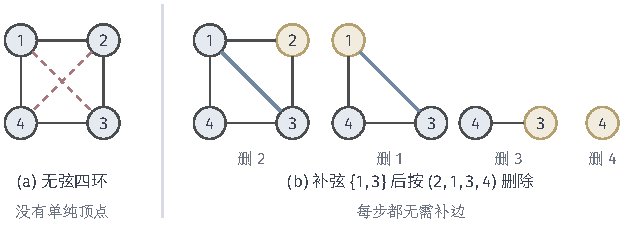
\includegraphics[width=106.306mm]{figures/01-basic-mathematics/04-graphs/tikz/c5-chordal-four-cycle/figure.pdf}
  \caption{无弦四环与补弦后的图。左：四环中每个顶点的两个邻居都不相邻（红色虚线为所缺的边），没有单纯顶点。右：补入弦$\{1,3\}$（蓝色）后，按$(2,1,3,4)$逐个删除，每一步被删除的黄色顶点的剩余邻居都已相邻，全程无填充。}
  \label{fig:graph-dp-chordal-four-cycle}
\end{figure}

四环的问题出在“长度至少为四而没有捷径的环”。在长度至少为$4$的环上，连接两个在环上不相邻的顶点的边称为该环的\term{弦}（chord）。每个长度至少为$4$的环都有弦的有限无向图称为\term{弦图}（chordal graph）。树没有环，是弦图；补入$\{1,3\}$后的四环是弦图；无弦四环不是。给一般图补边使之成为弦图称为\term{弦化}（chordal completion）。任何消元次序补边后的图都是弦图，因为该次序就是补边后图的完美消元序，由下面的定理即知；所以第一小节的构造实际上隐含了一次弦化。

\begin{theorem}[弦图与完美消元序]
\label{thm:graph-dp-chordal-peo}
有限无向图是弦图，当且仅当它有完美消元序。
\end{theorem}

\begin{proof}
先证有完美消元序的图是弦图。设图中有长度至少为$4$且无弦的环，考察环上最先被处理的顶点$v$。$v$在环上的两个邻居$u,w$此时都还在图中，并且与$v$相邻。$v$是单纯顶点，所以$u,w$相邻；而沿完美消元序处理时从不补边，$\{u,w\}$必是原图的边。环长至少为$4$，$u,w$在环上不相邻，于是$\{u,w\}$是这个环的弦，矛盾。

反方向的论证路线如下。第一步是一个引理：每个非空有限弦图都有单纯顶点，若它不是完全图，还有两个不相邻的单纯顶点。这一步需要分析极小分隔集，证明极小分隔集在弦图中都是团，本书不展开。第二步，弦图的诱导子图仍是弦图，因为诱导子图中的无弦环在原图中也无弦。于是可以反复删去一个单纯顶点，余下的图仍是弦图、仍有单纯顶点，直到删完，删除的次序就是完美消元序。
\end{proof}

\paragraph{构造与核验}
定理只说明弦图有完美消元序，并没有给出高效的求法。最直接的构造是逐次寻找单纯顶点：在当前图中按编号检查每个顶点，枚举它的每对邻居看是否相邻，找到第一个单纯顶点就删去它并追加到次序中；若非空的当前图中找不到单纯顶点，就报告输入不是弦图，并返回这个当前图作为证据，而不暗中补边。每轮最多检查$n$个顶点，检查顶点$v$需要$O(|N(v)|^2)$次查边，直接实现的总检查量最坏可达$O(n^4)$。存在线性时间的专门算法，这里不展开。

构造得到的次序应当独立核验。给定原图和一个次序，先确认它恰好包含每个顶点一次，再为每个顶点记下次序位置；对每个$v$取出原图中排在它之后的邻居，检查它们是否两两相邻。全部通过时次序是完美消元序，因为在不补边的前提下，处理$v$时的当前邻居恰好就是这些后续邻居；发现缺边时，就把$v$和那对不相邻的邻居作为失败证据返回。核验的检查量为$O(n+m)$再加$\sum_v|N^+_\pi(v)|^2$次查边。例如把$(2,1,3,4)$用于无弦四环，第一个顶点$2$的后续邻居$\{1,3\}$不相邻，立即被拒绝；用于补弦后的图则通过。

\paragraph{极大团与最大团}
弦图上可以直接用团作袋，这需要区分两种“最大”。不能再加入任何其他顶点而保持两两相邻的团称为\term{极大团}（maximal clique），这是按集合包含判断的；在所有团中顶点数最多的称为\term{最大团}（maximum clique）。例如三角形$1,2,3$外加一条边$\{3,4\}$，极大团是$\{1,2,3\}$和$\{3,4\}$；后者不能再扩大，但只有两个顶点，不是最大团。下面的团树需要全部极大团，而不只是最大的几个。

\subsection{团树的构造}

以弦图的全部极大团为袋、并满足运行交集的树分解称为\term{团树}（junction tree，也称clique tree）。团树中每个袋都是团，没有因填充而多出的变量，相邻两袋的交集就是它们共享的变量。本小节回答两个问题：怎样从完美消元序得到全部极大团；怎样把它们连成满足运行交集的树。

\paragraph{从完美消元序得到极大团}
设$\pi$是已经核验的完美消元序。对每个顶点$v$，候选集合$K_v=\{v\}\cup N^+_\pi(v)$是团，因为$v$被处理时是单纯顶点。反过来，任一团$C$都包含在某个$K_v$中：取$C$中最先被处理的顶点$v$，$C$的其余顶点都在$v$之后且与$v$相邻，所以都属于$N^+_\pi(v)$。因此极大团恰好是候选集合中不被其他候选严格包含的那些。具体做法是：生成全部$K_v$，删去重复的集合，再删去被其他候选严格包含的集合。

图~\ref{fig:graph-dp-clique-tree-mst}的弦图有边$\{1,2\},\allowbreak\{1,3\},\allowbreak\{2,3\},\allowbreak\{2,4\},\allowbreak\{3,4\},\allowbreak\{3,5\},\allowbreak\{4,5\}$，$(1,2,5,3,4)$是它的完美消元序。候选集合为$K_1=\{1,2,3\}$、$K_2=\{2,3,4\}$、$K_5=\{3,4,5\}$、$K_3=\{3,4\}$、$K_4=\{4\}$；删去被包含的$K_3,K_4$，得到三个极大团$A=\{1,2,3\}$、$B=\{2,3,4\}$、$C=\{3,4,5\}$。

\paragraph{用最大权生成树连接}
直觉上，共享变量多的团应该相邻，这样接口才能携带足够的共同变量。在以极大团为顶点的完全图上，给每对团$C,D$赋权$w(C,D)=|C\cap D|$，交集为空的零权边也保留；然后求这个图的最大权生成树，可以把权取负后调用第~\ref{sec:graph-minimum-spanning-tree}节的Kruskal或Prim方法。上例中$w(A,B)=2$、$w(B,C)=2$、$w(A,C)=1$，最大权生成树是$A-B-C$，总权为$4$。若改选$A-B$与$A-C$，总权为$3$，此时含$4$的两个团$B,C$之间隔着不含$4$的$A$，运行交集被破坏，如图~\ref{fig:graph-dp-clique-tree-mst}右侧所示。

\begin{figure}[!htb]
  \centering
  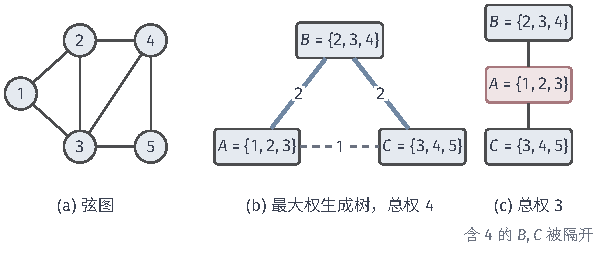
\includegraphics[width=102.306mm]{figures/01-basic-mathematics/04-graphs/tikz/c5-clique-tree-mst/figure.pdf}
  \caption{用交集权重的最大权生成树连接极大团。左：弦图。中：三个极大团组成的候选完全图，边上的数是交集大小，蓝色粗线是总权为$4$的最大权生成树$A-B-C$，虚线是未被选中的候选边。右：总权为$3$的另一棵生成树$B-A-C$，含$4$的团$B,C$被不含$4$的$A$（红色）隔开，不满足运行交集。}
  \label{fig:graph-dp-clique-tree-mst}
\end{figure}

下面的定理说明，这个例子中的对应关系是一般的。

\begin{theorem}[团树与最大权生成树]
\label{thm:graph-dp-clique-tree-mst}
设$\mathcal H$是非空有限弦图，$\mathcal C$是它的全部极大团。在以$\mathcal C$为顶点的完全图上令$w(C,D)=|C\cap D|$。则一棵生成树满足运行交集，当且仅当它的总权最大。
\end{theorem}

\begin{proof}
先给出任意生成树的总权上界。对生成树$\mathcal T'$，把每条边的权按共享变量拆开计数：
\[
\sum_{\{C,D\}\in\mathcal T'}|C\cap D|=\sum_{v}e_v,
\]
其中$e_v$是两端都含$v$的树边条数。设$v$属于$r_v$个极大团，两端都含$v$的树边正是$\mathcal T'$在这$r_v$个节点上的诱导子图的边；树的诱导子图没有环，是$r_v$个节点上的森林，所以$e_v\leq r_v-1$，且等号成立当且仅当这个诱导子图连通，即含$v$的团在$\mathcal T'$中连通。于是总权不超过$\sum_v(r_v-1)$，等号成立当且仅当对每个$v$都满足运行交集。

剩下要证明确实存在满足运行交集的生成树，即团树存在；那时最大总权恰为$\sum_v(r_v-1)$，最大权生成树就是满足运行交集的生成树。取一个完美消元序，按定理~\ref{thm:graph-dp-elimination-decomposition}的方法以$K_v$为袋得到树分解。若某个袋包含于相邻的袋，就把这条袋树边收缩，只保留较大的袋：顶点覆盖和边覆盖不受影响；对运行交集，被收缩的较小袋中的变量都在较大袋中，收缩一条两端都含$v$的边不破坏$T_v$的连通性，而不含$v$的较小袋本来不在$T_v$中，收缩后$T_v$也不变。反复收缩，直到没有相邻两袋有包含关系。这时任何两个袋都没有包含关系：若$B_s\subseteq B_t$而$s,t$不相邻，取路径上与$s$相邻的节点$s'$，由运行交集$B_s$的每个变量都在$B_{s'}$中，与“相邻袋无包含关系”矛盾。各袋都是团且互不包含；每个极大团都被某个袋容纳（引理~\ref{lem:graph-dp-clique-in-bag}），而袋本身是团，所以二者相等；每个袋也都是某个极大团，否则它会被那个极大团所在的另一个袋严格包含。于是剩下的袋恰好是全部极大团，各出现一次，团树存在。
\end{proof}

在上例中，$r_1=1$、$r_2=2$、$r_3=3$、$r_4=2$、$r_5=1$，上界$\sum_v(r_v-1)=4$，正好等于$A-B-C$的总权。不连通的弦图中，不同分量的团之间交集为空，零权边只用于把各分量的团树连成一棵树，不影响上界。

\paragraph{适用范围与结果核对}
定理要求输入是弦图，并且使用全部极大团。对无弦四环，极大团是四条边$\{1,2\},\allowbreak\{2,3\},\allowbreak\{3,4\},\allowbreak\{1,4\}$，每个顶点属于两个团；要让每个顶点的两个团相邻，需要四条树边，而四个节点的树只有三条边，所以任何生成树都不满足运行交集。一般图应先弦化，例如用某个消元次序补边，再在弦化后的图上构造团树；在原图的极大团上任选一棵树并不能保证得到树分解。选哪一种弦化决定了袋的大小，而团树构造只负责连接给定弦图的团，不负责找最好的弦化。

最大权生成树依赖上面的定理才保证运行交集，因此输出后仍应逐个顶点检查含它的团是否连通，作为对输入是否为弦图、团列表是否完整的独立核对。开销方面，设极大团有$p$个，候选完全图有$p(p-1)/2$条边，每条边的权需要一次集合求交；排序与并查集的开销按第~\ref{sec:graph-minimum-spanning-tree}节的分析计算。弦图的极大团数不超过顶点数$n$，因为每个极大团都是某个$K_v$。
